\section{Software}

\subsection{Generel struktur}

\subsection{Kommunikations Protokol}
I oplægget er der specificeret en kommunikationsprotokol som bilen skal overholde. Protokollen fungerer ved hjælp af telegrammer. I afsnittet "Beskrivelse af telegram" forklares der, hvad et telegram er. Og i afsnittet "Implementering" beskrives der, hvordan protokollen kodemæssigt er implementeret i microcontrolleren.

\subsubsection{Beskrivelse af telegram}
Protokollen er baseret på "telegrammer" bestående af 3 bytes der henholdsvis repræsenterer en type, kommando og et parameter.\\
Af typer er der specificeret 3 forskellige:
\begin{itemize}
	\item SET - 0x55 - Bruges til at sætte en værdi i bilen
	\item GET - 0xAA - Bruges til at hente en værdi fra bilen
	\item REPLY - 0xBB - Bruges til når der returneres en værdi som svar på et get/set telegram
\end{itemize}
Det har ikke været nødvendigt at implementerer yderligere typer, så dette er også de eneste tre typer som implementeringen gør brug af.\\
Af kommandoer er der fra oplæggets side sat et krav om to som bilen som minimum skal overholde, disse er som følger:
\begin{itemize}
	\item Start - 0x10 - Bruges til at starte bilen med en procentdel af maxspændingen ud 			fra parametret
	\item Stop - 0x11 - Bruges til at stoppe bilen med
\end{itemize}

Ud over dette har vi specificeret yderligerer to set kommandoer:
\begin{itemize}
	\item Speed\_H - 0x12 - Bruges til at sætte de øverste 8 bit af en 16-bit værdi der essentielt bestemmer hvilken hastighed hastighedskontrollen forsøger at holde
	\item Speed\_L - 0x13 - Bruges til at sætte de nederste 8 bit af en 16-bit værdi der essentielt bestemmer hvilken hastighed hastighedskontrollen forsøger at holde
\end{itemize}

Disse to kommandoer er essentielt en kommando, men skal sendes som to seperate kommandoer da et telegram kun kan bestå af en type, kommando og et parameter. De er blevet brugt meget til at teste hastighedskontrollen af og fastsætte max hastigheder rundt i forskellige sving.\\

Fra oplæggets side er der ikke specificeret nogle get kommandoer, men vi har implementeret de følgende:
\begin{itemize}
	\item Xaccel\_H - 0xA1 - Returner de øverste 8 bit af den signerede 16-bit rå værdi fra acceleration af x-aksen på sensoren
	\item Xaccel\_L - 0xA2 - Returner de nederste 8 bit af den signerede 16-bit rå værdi fra acceleration af x-aksen på sensoren
	\item Zgyro\_H - 0xA3 - Returner de øverste 8 bit af den signerede 16-bit rå værdi af vinkelhastigheden om z-aksen på sensoren
	\item Zgyro\_L - 0xA4 - Returner de nederste 8 bit af den signerede 16-bit rå værdi af vinkelhastigheden om z-aksen på sensoren
	\item Ticks\_H - 0xA5 - Returner de øverste 8 bit af den 16-bit værdi der fortæller, hvor mange "ticks" bilen har kørt på daværende tidspunkt
	\item Ticks\_L - 0xA6 - Returner de nederste 8 bit af den 16-bit værdi der fortæller, hvor mange "ticks" bilen har kørt på daværende tidspunkt
	\item LapTime\_H - 0xA7 - Returner de øverste 8 bit af den 16-bit værdi der fortæller, hvor mange millisekunder banen tog at gennemfører
	\item LapTime\_L - 0xA8 - Returner de nederste 8 bit af den 16-bit værdi der fortæller, hvor mange millisekunder banen tog at gennemfører
	\item LapTicks\_H - 0xA9 - Returner de nederste 8 bit af den 16-bit værdi der fortæller, hvor mange "ticks" der har været på en omgang af banen
	\item LapTicks\_L - 0xAA - Returner de nederste 8 bit af den 16-bit værdi der fortæller, hvor mange "ticks" der har været på en omgang af banen
	\item Data - 0xAB - Bliver brugt til at få bilen til at returnerer flere data-værdier uden at skulle sende et get telegram for hver enkelt. Justeres ind alt efter hvad man gerne vil have tilbage.
	
\end{itemize}

Til sidst i telegrammet sendes der altid et parameter med, også selvom en funktion ikke gør brug af et parameter.

\subsubsection{Implementering}

\subsection{Eksempler(sensor)}

\subsubsection{Tachometer}

Til at behandle signalet fra hall sensoren, benyttes input capture funktionen til Timer 1. Input capture funktionen har sit eget interrupt og fungerer ved automatisk at læse værdien af Timer 1's timer/counter registre (TCNT1A/TCNT1B) over i to input capture registre (ICR1L/ICR1H) når der kommer et interrupt. Input capture er den sekundære funktion til PD6, og sættes op i Timer 1's kontrol registre (TCCR1A/TCCR1B). Vi valgte at sætte den op med en prescaler på 1/8 og en falling edge interrupt trigger. Det giver en opdateringsfrekvens på 0.5 $\mu s$ og en maksimal tid på 32.5 ms inden timer/counter registrene overflower. Det er fint nok til at kunne rumme tiden imellem flere interrupts. I interruptrutinen beregnes tiden imellem 4 interrupts for at finde ud af hvor lang tid motoren er om at dreje en omgang (Der sidder tre poler på motoren, så 4 interrupts vil svare til en hel omgang for motoren). Denne tid kan så bruges som et udtryk for hastigheden, da de to ting er omvendt proportionale. Bilens reelle hastighed kan også beregnes, men på grund af proportionaliteten er det ligegyldigt, fra microcontrolleren's synspunkt, om man bruger det ene eller det andet - man skal bare huske at en høj hastighed vil give en lav tid og omvendt, når man skriver programmet, der skal bearbejde hastigheden. Jo færre cycles man bruger på at få noget brugbart ud i den anden ende jo bedre, i næsten alle tilfælde, når der også skal laves andre ting sideløbende med input capture interruptet.\\
For at beregne tiden skal der holdes styr på pulserne - der skal bruges en tid fra den første puls og en tid fra den sidste puls. Det letteste er at tælle en variabel op, hver gang der modtages et interrupt således at, når variablen er 1 så læser man den første tid, og når variablen er 4 så læses den sidste tid. Derefter trækkes de to tider fra hinanden for at finde forskellen. Alle værdier og variable gemmes i SRAM-hukommelsen på tildelte addresser indtil de skal bruges igen.\\

Det viste sig at hall sensoren gav mange udslag når bilen holdt stille og en af polerne var lige på grænsen til at passere sensoren. Vi antager at det er fordi feltet er meget ustabilt i grænseområdet. 


\subsubsection{Lap sensor}

For at initialisere microcontrolleren's komparator skal den sættes op i dens eget status register (ACSR) og i Special Function IO Registret (SFIOR). Man kan vælge flere forskellige inputs til komparatoren - PB2(AIN1) og PB3(AIN0) er henholdsvis ikke-inverterende og inverterende inputs som standard. Alternativt kan hele PORTA bruges til det inverterende og den interne bandgap reference på 2.56 V til det ikke-inverterende.  ACME bit'en i SFIOR enabler ADC multiplexeren, så den styrer hvilket ben på PORTA der bliver brugt. ACBG bit'en enabler bandgap referencen.

\begin{figure}[h]

	\centering
		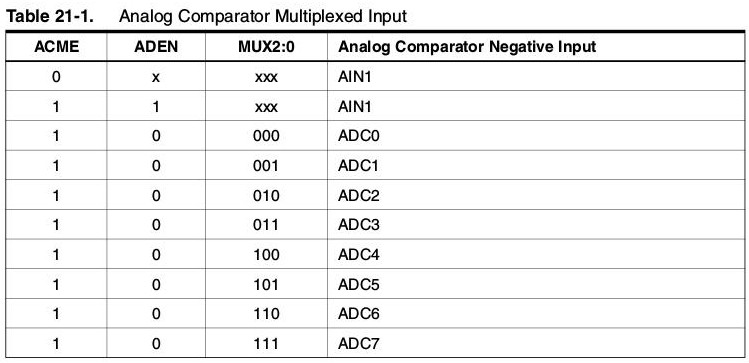
\includegraphics[scale=0.3]{Billeder/Table21-1.jpg}
	\caption{I tabellen kan man se at ACME bit'en lader multiplexeren vælge hvilket ben på PORTA, der er input til komparatorens inverterende ben. Medmindre ADC'en er slået til - så bliver inputtet taget fra PB2(AIN1)}
	\label{fig:ACME}
	
\end{figure}

Man har også mulighed for at vælge, hvornår komparatoren skal sende et interrupt. Interruptet bliver sendt som en reaktion på hvad der sker på komparatorens output-ben. Vi har sat den op til at sende et interrupt, når outputtet toggler tilstand, men der er også mulighed for at køre på enten falling eller rising edge. Det betyder i vores tilfælde ikke noget hvilken metode man vælger på grund af måden koden bearbejder interruptet, men mere om det senere.\\

I interruptrutinen til lap sensoren beregnes omgangstiden. Hver gang målstregen krydses læses tiden fra tre SRAM addresser, hvor tiden microcontrolleren har været tændt millisekunder er gemt i 24 bits. Interruptrutinen sørger for at gemme et 24 bits time stamp i SRAM'en hver gang den køres. Med den totale tid og et time stamp fra det forrige interrupt, er det bare et spørgsmål om at trække de to fra hinanden for at finde omgangstiden. For at forhindre ugyldige omgangstider, hvis der kommer mere end et interrupt på samme målstreg, kontrolleres det om omgangstiden er længere end 512 millisekunder se figur \ref{fig:LapTime}.

\begin{figure}[h]

	\centering
		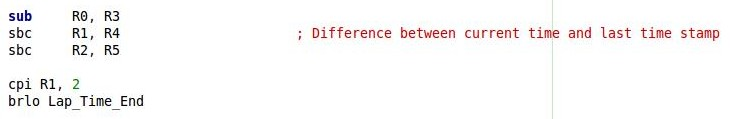
\includegraphics[scale=0.5]{Billeder/LapTime.jpg}
	\caption{Her er den nuværende tid gemt i R0, R1, R2 og time stampet i R3, R4, R5. Ved at kontrollere om den mellemste byte i R1 er under 2 kan det afgøres, om der er gået nok tid siden sidste time stamp til at anse interruptet som gyldigt.}
	\label{fig:LapTime}
	
\end{figure}

Det er også efter denne kontrol at man kan ændre på alle de parametre der kun skal ændres en gang når målstregen krydses. Inden man forlader interruptrutinen er det vigtigt at resette comparator interrupt flaget i ACSR. Hvis flaget er sat, når det globale interrupt bliver enablet efter rutinen, anser microcontrolleren det som om den har modtaget et nyt interrupt, og så vil den køre hele rutinen igen.

\subsection{Hastighedskontrol}


\subsection{AI}

\subsection{GUI}
